\documentclass[aspectratio=169,11pt,hyperref={colorlinks=true}]{beamer}
\usepackage[utf8]{inputenc}
\usepackage[T1]{fontenc}
\usepackage{fontspec}
\usepackage[absolute,overlay]{textpos}
\usepackage{listingsutf8}
\usepackage{listings-golang}
\usepackage{tikz}
\usepackage{color}
\usepackage{fontawesome5}
\usepackage{svg}


\title{Adopting CDEvents and Embracing Interoperability}
\date[19 September 2024]{CD Mini Summit @ OSSEU | 19 September 2024 | \faTwitter ~@\_cdevents | \faGithub ~cdevents}
\author[Andrea Frittoli]{%
  Andrea Frittoli \\
  Developer Advocate @ IBM\\
  andrea.frittoli@uk.ibm.com \\
  \faTwitter ~@blackchip76 | \faGithub ~afrittoli\\
  ~\\
  Session: \href{https://sched.co/1aBN2}{sched.co/1aBN2}
}

\usetheme{af}

% Code style
\setlststyle

\lstdefinelanguage{koyaml}{
  keywords={github, com, afrittoli, examples, ms, go, helloworld},
  sensitive=false,
  comment=[l]{\#},
  morestring=[b]',
  morestring=[b]"
}

% Automatic section frame
% \AtBeginSection{\frame{\sectionpage}}

\begin{document}

\begin{frame}
\titlepage{}
\end{frame}

\begin{speakerframe}[af_wind.jpg]{Andrea Frittoli}%
  {%
  \faGithub ~afrittoli | \faLinkedin ~andreafrittoli | \faTwitter ~@blackchip76
  }%
  {%
  \begin{itemize}
    \item{Open Source Advocate @ IBM}
    \item{Lives in Wales, enjoys the wind}
    \item{CDEvents maintainer, Events SIG co-chair}
    \item{Chair of CDF Technical Oversight Committee \\ Governing Board}
  \end{itemize}
  }%
\end{speakerframe}

\begin{lpicrblack}[calum-lewis-vA1L1jRTM70-unsplash.jpg]{%
  Photo by \href{https://unsplash.com/@calumlewis}{\underline{Calum Lewis}}, CC0
  }%
  {%
  \tableofcontents
  }%
  {}
  \frametitle{~~~~~~~~~~~~~~~~~~~~~~~~~~~~~~~~~~~~~~~~~~~~~~~~~~~Contents}
\end{lpicrblack}

\section[Software Factory]{Software Factory}

\begin{sectionwithpiclargecentral}[jezael-melgoza-HYQvV8wWX18-unsplash.jpg]{Photo by \href{https://unsplash.com/@jezar}{\underline{Jezael Melgoza}}, CC0}
\end{sectionwithpiclargecentral}
  \note[itemize]{
    \item Building Software
  }

\begin{blackframe}
  \frametitle{Software Factory}
  \begin{itemize}
    \item "Glue code" explosion
    \item Does not scale
    \item Expensive to onboard \\new services
    \item Hard to maintain
  \end{itemize}
  \begin{textblock*}{0.60\paperwidth}(0.35\paperwidth,0.13\paperheight)
    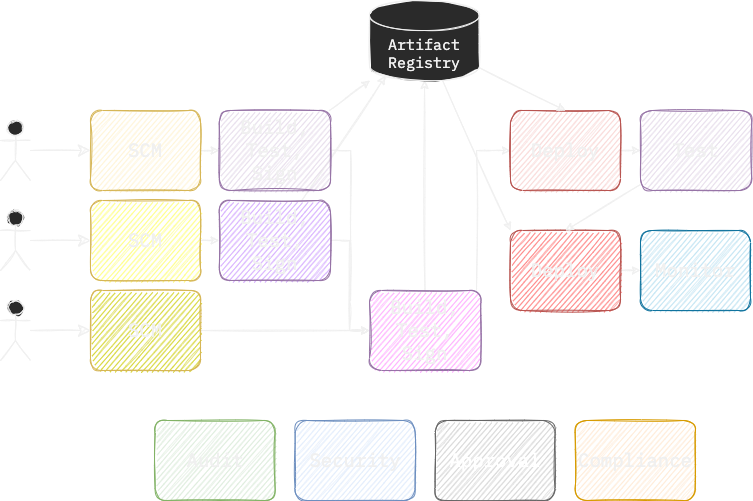
\includegraphics[width=0.60\paperwidth]{img/cdevents-multiple-components.png}
  \end{textblock*}
\end{blackframe}
\note[itemize]{
  \item 2. Multiple components, more requirements (glue code)
  \item Use existing diagrams, the second diagram from the google slides version
}

\begin{blackframe}
  \frametitle{Internal Development Platform}
  \begin{itemize}
    \item Lock-in effect
    \item Missing/Broken Data
    \item Many Dashboards
  \end{itemize}
  \begin{textblock*}{0.60\paperwidth}(0.35\paperwidth,0.13\paperheight)
    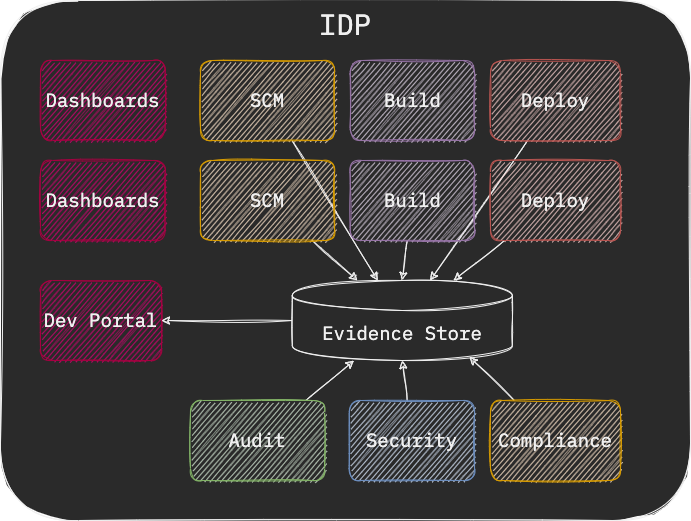
\includegraphics[width=0.60\paperwidth]{img/cdevents-idp-multiple.png}
  \end{textblock*}
\end{blackframe}
\note[itemize]{
  \item 2. Multiple triggers, 1 dashboard, evidence store (metrics, audit)
  \item Draw two diagrams with IDP
}

\begin{grayframe}
  \frametitle{A Plethora of Tools}
  \begin{textblock*}{1.0\paperwidth}(0\paperwidth,0.18\paperheight)
    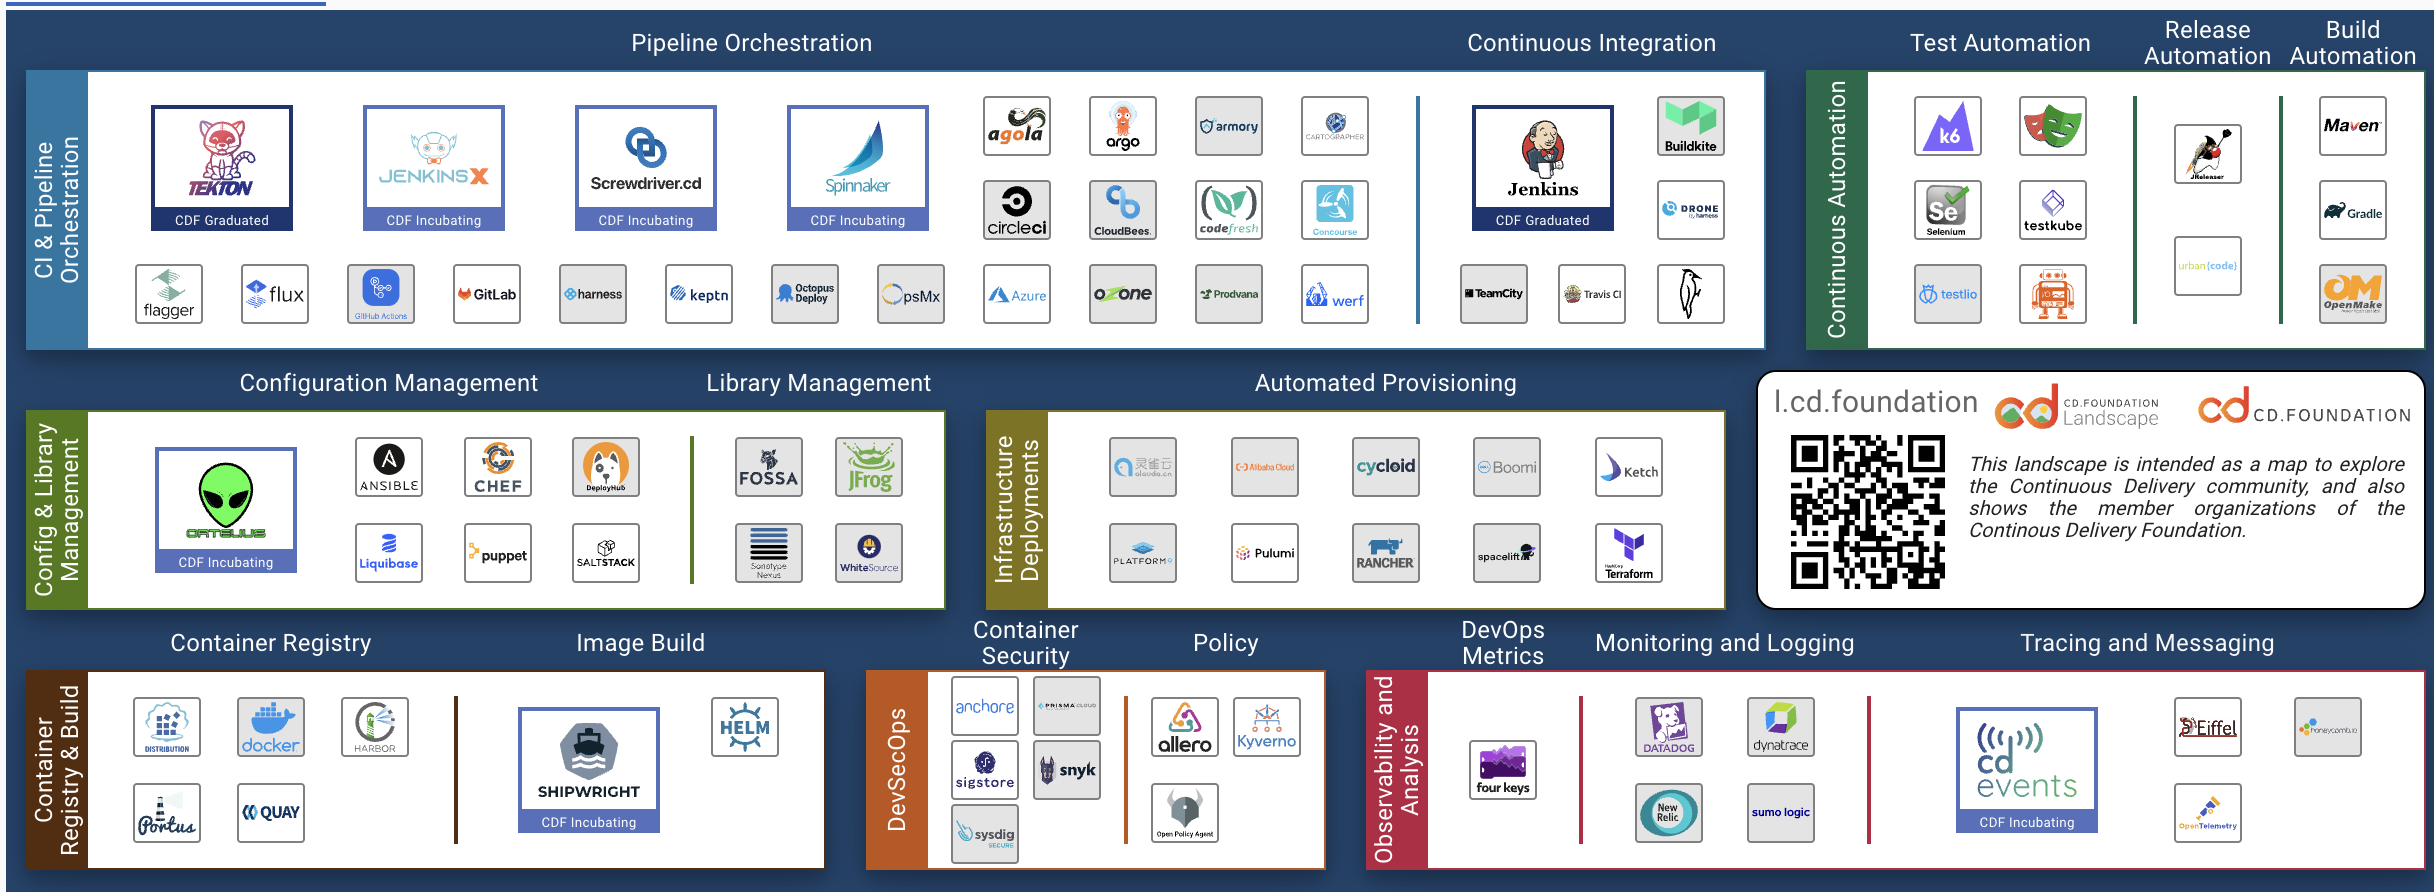
\includegraphics[width=1.0\paperwidth]{img/landscape.cd.foundation.png}
  \end{textblock*}
\end{grayframe}
\note[itemize]{
  \item We need multiple tools to satisfy requirements, improve metrics
  \item Added complexity, risk, skills required
  \item We need data to satisfy requirements
  \item Mention slashdata report
  \item Use the landscape diagram
}

\section[CDEvents]{A common specification for Continuous Delivery Events}

\begin{sectionwithpicmediumcentral}[cdeventscon-gradient-16-9.jpg]{
  \begin{textblock*}{0.07\paperwidth}(0.88\paperwidth,0.89\paperheight)
    
\includegraphics[width=0.07\paperwidth]{img/cdf-stacked-color.png}
  \end{textblock*}
}
\end{sectionwithpicmediumcentral}
\note[itemize]{
  \item How many of you are familiar with CDEvents?
}

\begin{grayframe}
  \frametitle{Interoperability}
  \begin{itemize}
    \item Less "Glue Code"
    \item More focus on DevEx \\
          and DevOps metrics
    \item Better quality data
    \item Drive Best Practices
  \end{itemize}
  \begin{textblock*}{0.60\paperwidth}(0.35\paperwidth,0.13\paperheight)
    \includegraphics[width=0.60\paperwidth]{img/cdevents-4-Interoperability.png}
  \end{textblock*}
\end{grayframe}

\begin{textondarkpic}[anthony-yin-okEUu6AMO2Y-unsplash]{%
  Photo by \href{https://unsplash.com/@anthonyin}{\underline{Anthony Yin}}, CC0
  }%
  \frametitle{Evidence Store\\Supply Chain Security}
  \begin{itemize}
    \item Where is this code deployed?\\
          ~~Tracking vulnerabilities\\~
    \item How was this code built?\\
          ~~Audit and compliance\\~
    \item How long did it take?\\
          ~~DevOps Metrics\\~
    \item What's happening right now?\\
          ~~One overview dashboard for all needs
  \end{itemize}
\end{textondarkpic}
\note[itemize]{
  \item Multiple dashboards -> Single point of entry. Backstage example. (Notifications?)
  \item Tracking vulnerabilities
  \item Audit and compliance
  \item Metrics
}

\begin{grayframe}
  \frametitle{IDP and CDEvents}
  \begin{itemize}
    \item Add/swap tools
    \item Consistent Data
    \item Single Dashboard
  \end{itemize}
  ~ \\
  \begin{itemize}
    \item Promotes Collaboration \\
          through Open Source
    \item CDEvents and \href{https://cnoe.io}{CNOE.io}
  \end{itemize}
  \begin{textblock*}{0.60\paperwidth}(0.35\paperwidth,0.13\paperheight)
    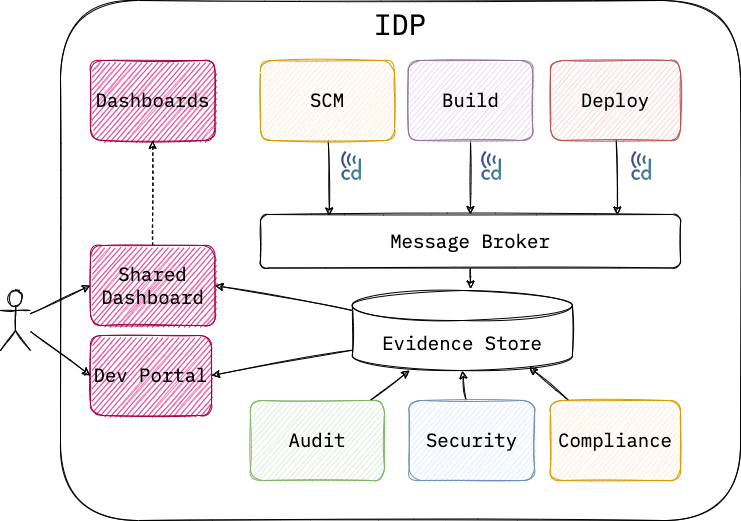
\includegraphics[width=0.60\paperwidth]{img/cdevents-idp-cdevents.png}
  \end{textblock*}
\end{grayframe}
\note[itemize]{
  \item From custom solutions to Open Source
  \item CNOE example, switch and combine tools
}

\begin{grayframe}
  \frametitle{Components}
  \begin{textblock*}{0.80\paperwidth}(0.10\paperwidth,0.15\paperheight)
    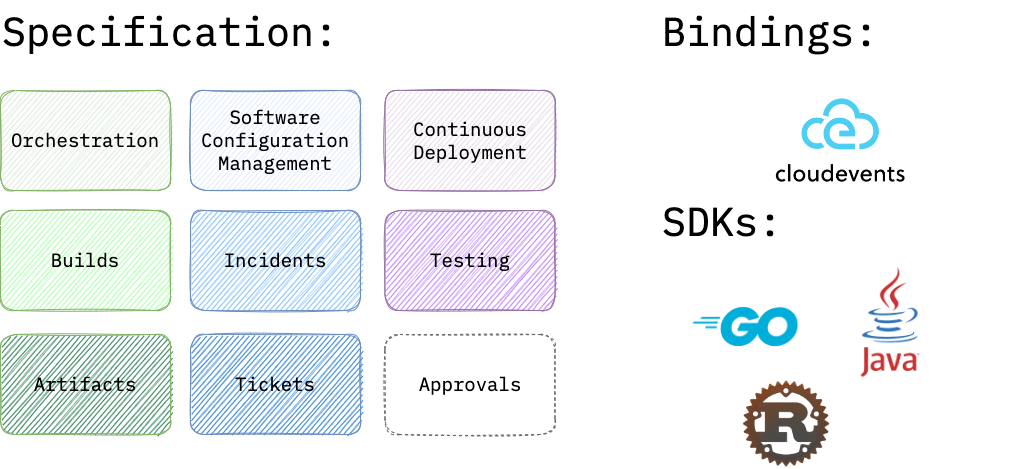
\includegraphics[width=0.80\paperwidth]{img/cdevents-components.png}
  \end{textblock*}
\end{grayframe}

\begin{blackframe}
  \frametitle{Community}
  \begin{itemize}
    \item DevOps Engineers\\
            ~~Share your Interoperability pain-points\\~
    \item Tool Maintainer\\
            ~~Adopt CDEvents for your tool\\~
    \item DevOps Vendor\\
            ~~Make it easier for users to integrate\\
            ~~your offering by supporting CDEvents\\~
    \item Love DevOps \& Interoperability\\
            ~~Join us and contribute to CDEvents!
  \end{itemize}
  \begin{textblock*}{0.45\paperwidth}(0.50\paperwidth,0.18\paperheight)
    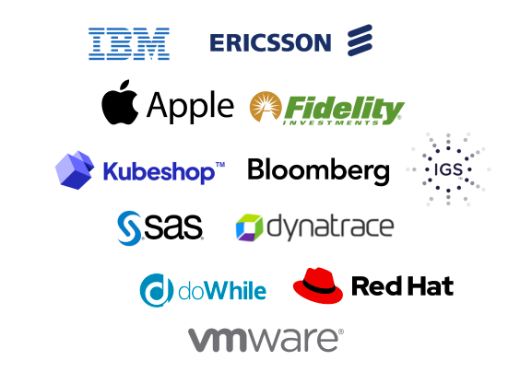
\includegraphics[width=0.45\paperwidth]{img/cdevents-community.png}
  \end{textblock*}
\end{blackframe}

% \section{Tools Adoption}
% \begin{sectionwithpiclargecentral}[clay-banks-LjqARJaJotc-unsplash.jpg]{Photo by \href{https://unsplash.com/@claybanks}{\underline{Clay Banks}}, CC0}
% \end{sectionwithpiclargecentral}

% \begin{3squares}{Overview}{%
%     CDF Projects:
%     \begin{itemize}
%       \item Jenkins
%       \item Spinnaker
%       \item Tekton (Experimental)
%     \end{itemize}
%     ~ \\
%     ~ \\
%     ~ \\
%   }{%
%   Other Projects:
%   \begin{itemize}
%     \item JReleaser
%     \item Guah.sh (OpenSSF)
%   \end{itemize}
%   }{%
%   CNCF Projects:
%   \begin{itemize}
%     \item Testkube
%     \item Flux
%     \item Argo CD (POC through Notifications)
%     \item Harbour (POC)
%   \end{itemize}
%   ~ \\
%   ~ \\
%   ~ \\
%   Planning:
%   \begin{itemize}
%     \item Ortelius
%     \item Updatecli
%   \end{itemize}
%   }
% \end{3squares}

% \begin{grayframe}
%   \frametitle{All Together}
%   \begin{textblock*}{0.60\paperwidth}(0.20\paperwidth,0.09\paperheight)
%     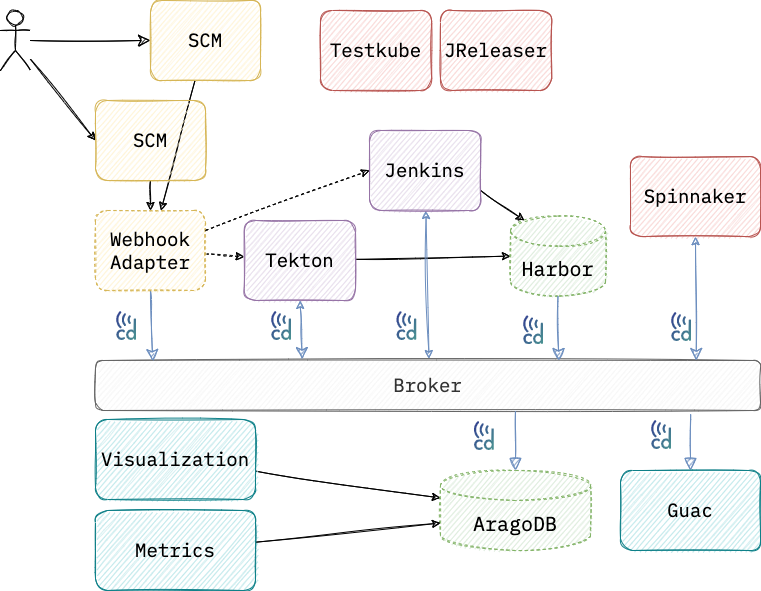
\includegraphics[width=0.60\paperwidth]{img/cdevents-poc.png}
%   \end{textblock*}
% \end{grayframe}

% \begin{3squares}{Successes and challenges}{%
%   Challenges:
%   \begin{itemize}
%     \item Grow the Community
%     \item Widespread Adoption
%     \item Culture
%   \end{itemize}
%   ~ \\
%   ~ \\
%   ~ \\
% }{%
% Success:
% \begin{itemize}
%   \item Widespread Interest
%   \item Tools Adoption
%   \item End Users
% \end{itemize}
% }{%
% Lessons Learnt:
% \begin{itemize}
%   \item Address specific pain point
%   \item Collaborations
% \end{itemize}
% ~ \\
% ~ \\
% ~ \\
% }
% \end{3squares}

% \begin{lpicrblack}[nick-fewings-ORSkFfgfEBI-unsplash.jpg]{%
%   Photo by \href{https://unsplash.com/@jannerboy62}{\underline{Nick Fewings}}, CC0
%   }%
%   {%
%   \begin{itemize}
%     \item OpenTelemetry:\\
%           ~~Semantics for Pipeline\\~~Observability
%   \end{itemize}
%   ~ \\
%   \begin{itemize}
%     \item \href{https://cnoe.io}{CNOE.io}:\\
%           ~~Interoperability layer for IDP
%   \end{itemize}
%   ~ \\
%   \begin{itemize}
%     \item Value Stream Management\\
%           Interoperability (VSMI) TC
%   \end{itemize}
%   }%
%   {0.35}
%   \frametitle{~~~~~~~~~~~~~~~~~~~~~~~~~~~~~~~~~~~~~~~~~~~~~~~~~~~Collaborations}
%   \begin{textblock*}{0.15\paperwidth}(0.83\paperwidth,0.25\paperheight)
%     \includegraphics[width=0.15\paperwidth]{img/cdevents-Collaborations.png}
%   \end{textblock*}
% \end{lpicrblack}

\section{What's New}
\begin{sectionwithpiclargecentral}[josh-sorenson-MjIMc6uhwrE-unsplash.jpg]{Photo by \href{https://unsplash.com/@joshsorenson}{\underline{Josh Sorenson}}, CC0}
\end{sectionwithpiclargecentral}

\begin{tpicstripedframe}%
  {cdevents-banner-v0-4.png}
  {%
  Linked Events:
  \vspace{0.01\textheight}
  \begin{itemize}
    \item Connect Events
    \item Fast Filtering
    \item Visualization
    \item Audit Trail
  \end{itemize}
  }%
  {%
  Ticket Events:
  \vspace{0.01\textheight}
  \begin{itemize}
    \item Inception to Deployment
    \item E2E Metrics
    \item Ticket Based Automation
    \item Interop.
  \end{itemize}
  }%
  {%
  Custom Events:
  \vspace{0.01\textheight}
  \begin{itemize}
    \item Schema
    \item Custom Types
  \end{itemize}
  \vspace{0.03\textheight}
  Artifact Events:
  \vspace{0.01\textheight}
  \begin{itemize}
    \item SBOM, User
    \item New Predicates
  \end{itemize}
  }%
  {%
  Release Announcement:
  \begin{textblock*}{0.17\paperwidth}(0.78\paperwidth,0.55\paperheight)
    
\includegraphics[width=0.17\paperwidth]{img/cdevents-v4-release-announcement.png}
  \end{textblock*}
  }%
\end{tpicstripedframe}
\note[itemize]{
  \item Update to v0.4 items, various slides
  \item 1. and 2. Content of release
  \item 3. Content of Release, Link to release, link to blog post
}

\begin{grayframe}
  \frametitle{What We're Working On}
  \begin{itemize}
    \item Webhook Adapter (list of plugins)
    \item GitHub Application
    \item Implementation Working Group (messaging service, software stack, specific use cases)
  \end{itemize}
\end{grayframe}

\section{Roadmap}
\begin{sectionwithpiclargecentral}[dimitar-donovski-yrjB4dYWUZU-unsplash.jpg]{Photo by \href{https://unsplash.com/@dmtrdon}{\underline{Dimitar Donovski}}, CC0}
\end{sectionwithpiclargecentral}

\begin{stripedframe}%
  {%
  CDEvents Roadmap \\
  v0.5 and beyond \\
  ~
  }%
  {%
  New features
  \vspace{0.02\textheight}
  \begin{itemize}
    \item Approvals
    \item Compositions
    \item Releases
  \end{itemize}
  }%
  {%
  Software \& Architecture
  \vspace{0.02\textheight}
  \begin{itemize}
    \item SDKs (JS, .NET)
    \item Webhook Adapter
    \item Visualization
    \item Links Service
  \end{itemize}
  }%
  {%
  Proof of Concept
  \vspace{0.02\textheight}
  \begin{itemize}
    \item CDEvents + CNOE.io
    \item CDEvents Visualization
  \end{itemize}
  }%
  {%
  Continue to Drive Adoption
  }%
\end{stripedframe}

\begin{2columnsframe}{Conclusions}%
  {%
  \begin{itemize}
    \item Lack of Standardization in the\\
    Continuous Delivery Space
  \end{itemize}
  \vspace{0.22\textheight}
  ~~~\textbf{which means}
  \vspace{0.05\textheight}
  \begin{itemize}
    \item Complexity \& Costly integrations
    \item Risk of inconsistent and\\
          incomplete data
    \item Developer fatigue
  \end{itemize}
  }{%
  \begin{itemize}
    \item CDEvents is a common specification for Continuous Delivery Events
  \end{itemize}
  \vspace{0.22\textheight}
  ~~~\textbf{which means}
  \vspace{0.05\textheight}
  \begin{itemize}
    \item Standardization
    \item Flexibility \& Better DevEx
    \item Better supply chain security stance through data
  \end{itemize}
  }
\end{2columnsframe}

\section[Thank You]{Thank You!}

\begin{sectionwithpiclargecentral}[carl-jorgensen-5nrnxx_tWe8-unsplash.jpg]{Brecon Beacons, Wales, Photo by \href{https://unsplash.com/@scamartist}{\underline{Carl Jorgensen}}, CC0}
\end{sectionwithpiclargecentral}

\begin{blackframe}
  \frametitle{References}
  \begin{itemize}
    \item \href{https://cdevents.dev}{cdevents.dev, github.com/cdevents}
    \item \href{https://cd.foundation}{CDF: cd.foundation}
    \item \href{https://landscape.cd.foundation}{CDF Landscspe: landscape.cd.foundation}
    \item \href{https://github.com/afrittoli/cdevents_interoperability}{Slides: github.com/afrittoli/cdevents\_interoperability}
  \end{itemize}
  \vspace{0.02\textheight}
  \begin{itemize}
    \item \href{https://cd.foundation/blog/2024/04/16/cdevents-v04/}{Release Announcement: cd.foundation/blog/2024/04/16/cdevents-v04/}
  \end{itemize}
  \vspace{0.1\textheight}
  Andrea Frittoli | \href{mailto:andrea.frittoli@uk.ibm.com}{andrea.frittoli@uk.ibm.com} \\
  \faTwitter ~@blackchip76 | \faGithub ~afrittoli | \faLinkedin ~andreafrittoli
  \begin{textblock*}{0.15\paperwidth}(0.70\paperwidth,0.18\paperheight)
    
\includegraphics[width=0.15\paperwidth]{img/cdcon2024-slides.png}
  \end{textblock*}
\end{blackframe}

\end{document}
